\newpage
\section{Herausforderungen und Lösungen}
Während der Backend-Entwicklung mussten mehrere technische Hürden überwunden werden.

\subsection{Blockierende Operationen bei großen Dateien}
\textbf{Problem:} Die Verarbeitung großer PDF-Dateien (Textextraktion, Chunking, Embedding-Generierung) innerhalb des HTTP-Request-Zyklus führte zu langen Wartezeiten und Timeouts im Frontend.
\textbf{Lösung:} Einführung einer \texttt{BackgroundJobQueue}. Der Upload-Endpoint nimmt die Datei entgegen, speichert sie in MinIO und reiht nur eine \glqq{}Job-ID\grqq{} in die Queue ein, bevor er sofort \texttt{202 Accepted} zurückgibt. Ein Hintergrunddienst (\glqq{}Worker\grqq{}) arbeitet diese Queue asynchron ab (siehe Abbildung~\ref{fig:background_job_queue}).

\begin{figure}[H]
    \centering
    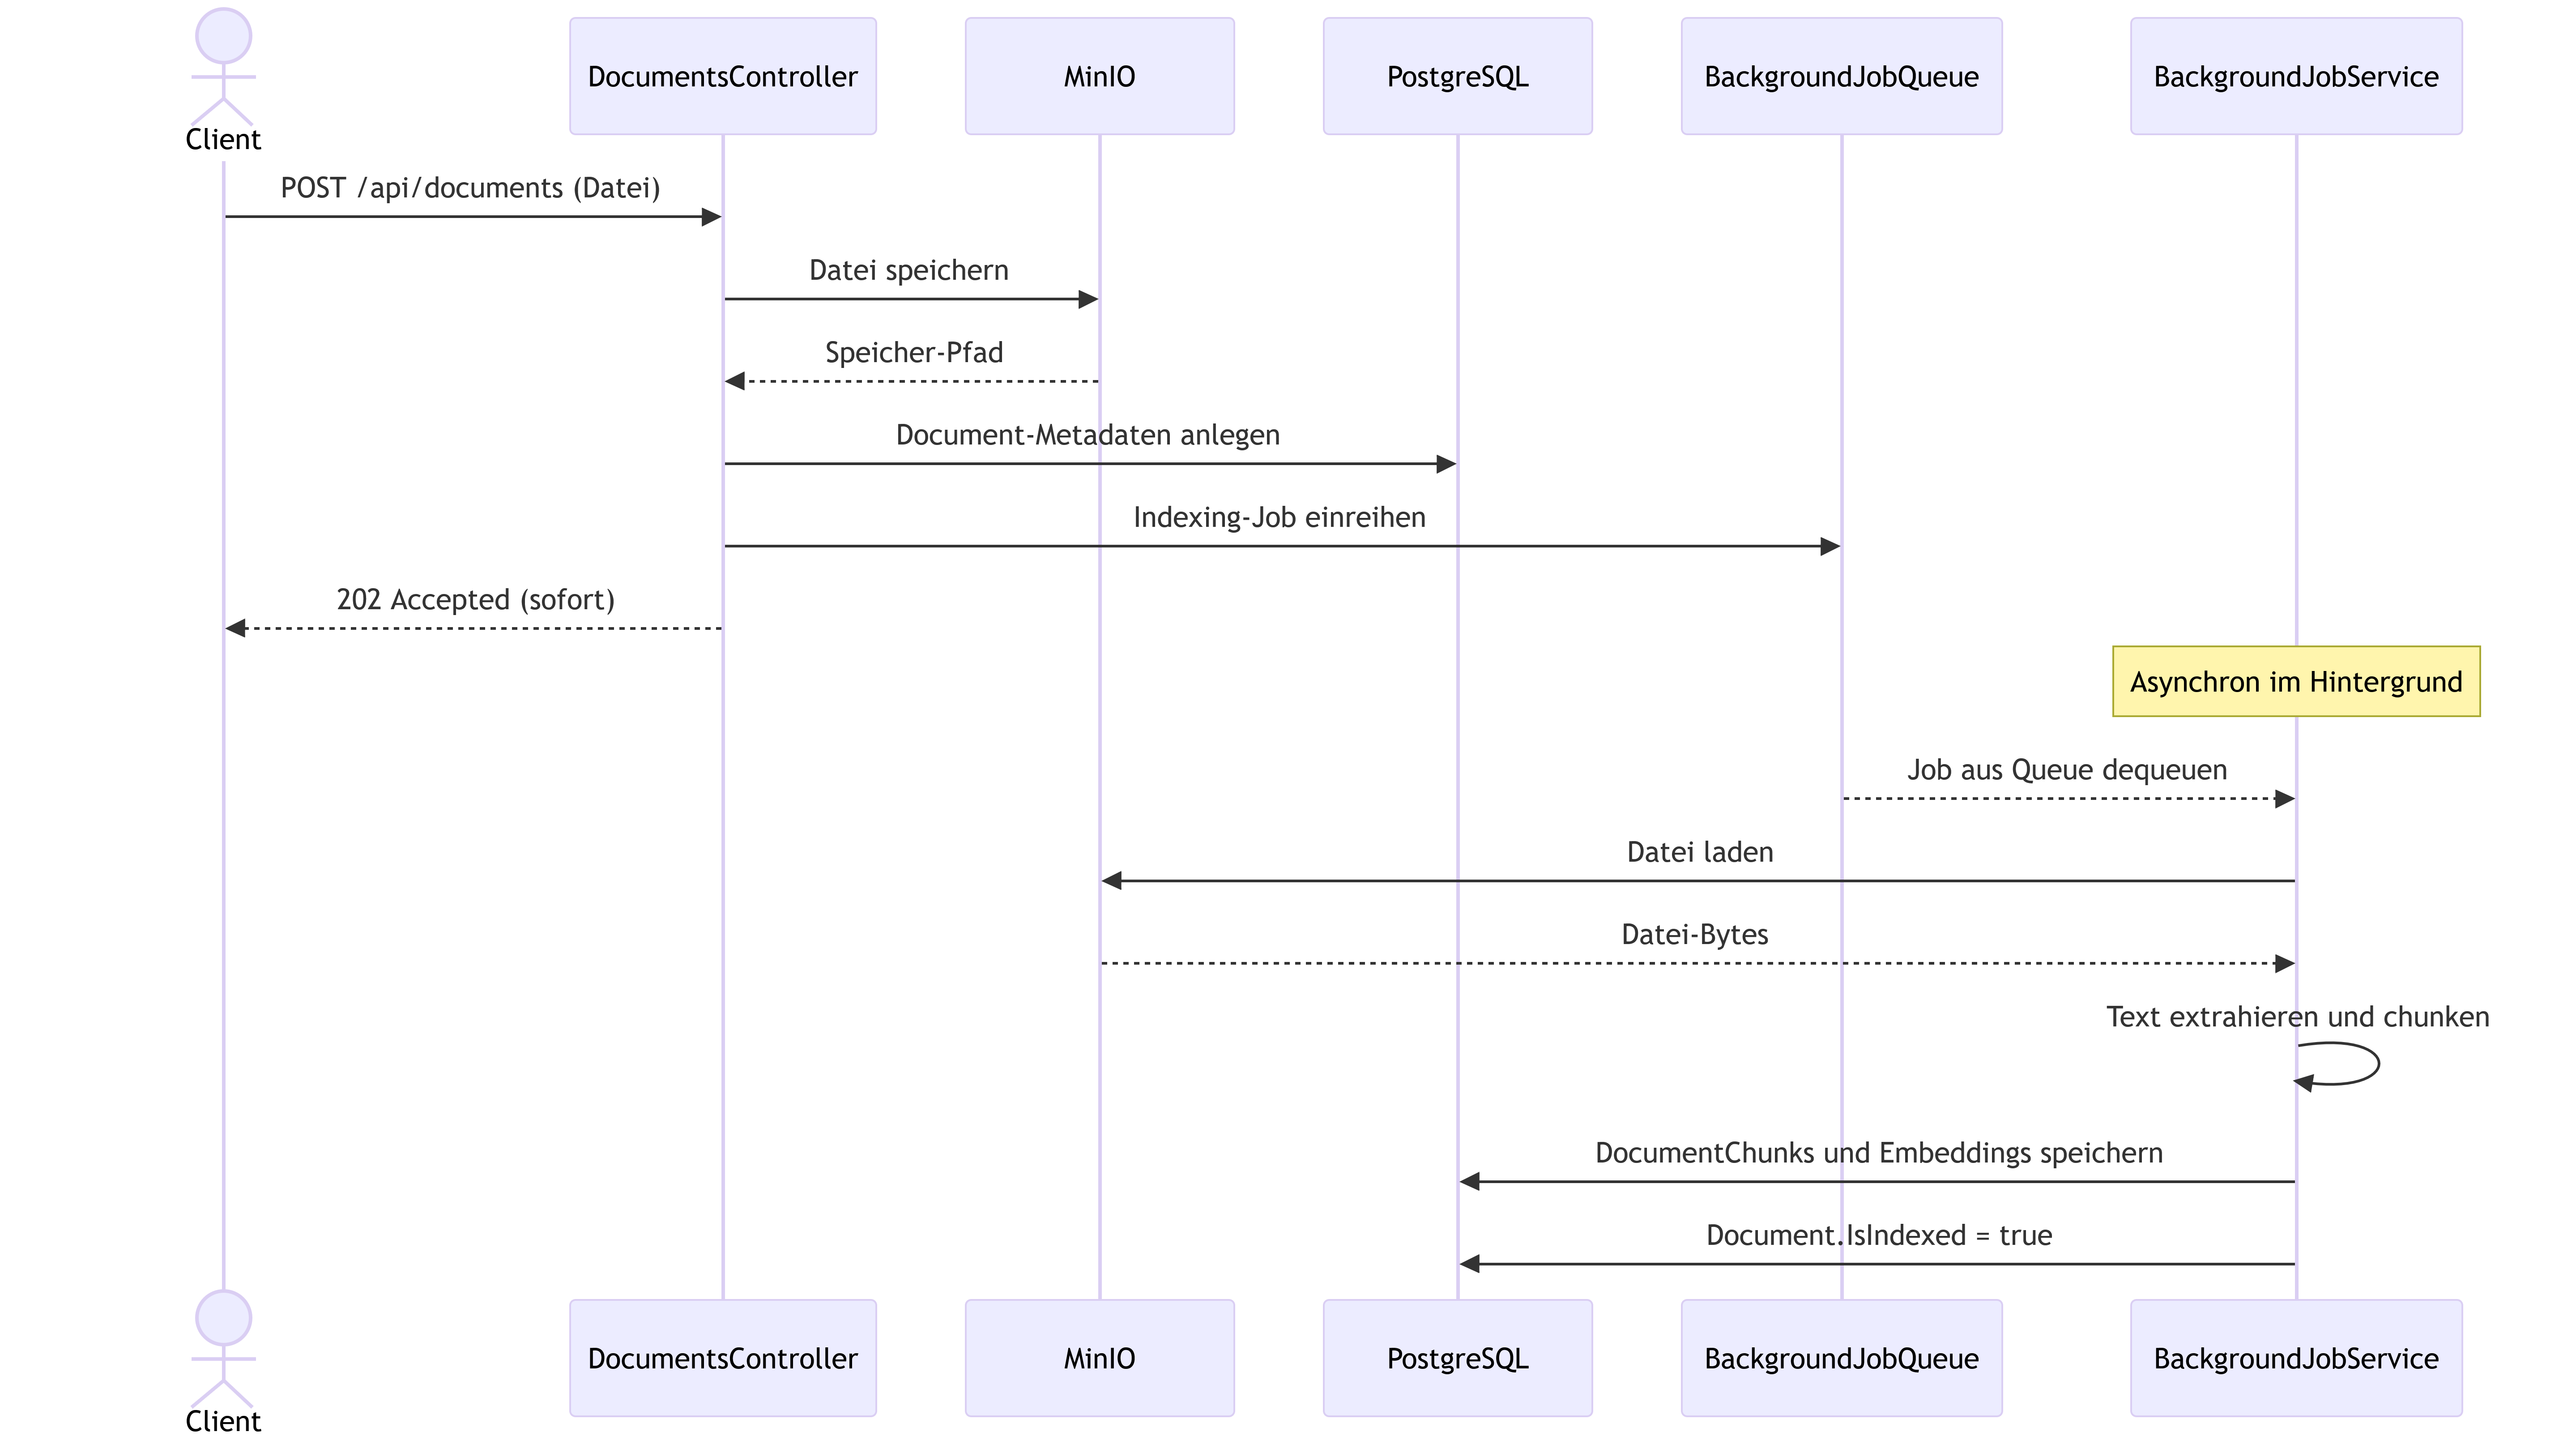
\includegraphics[width=\textwidth]{img/background_job_queue.png}
    \caption{Sequenzdiagramm des asynchronen Dokument-Upload-Flows}
    \label{fig:background_job_queue}
\end{figure}

\newpage
\begin{lstlisting}[language={[Sharp]C}, caption={Verarbeitungsschleife im BackgroundJobService}]
protected override async Task ExecuteAsync(CancellationToken stoppingToken)
{
    while (!stoppingToken.IsCancellationRequested)
    {
        var workItem = await _queue.DequeueAsync(stoppingToken); // Blockiert bis Arbeit da ist
        try
        {
            await workItem(stoppingToken); // Fuehrt den eigentlichen Indexing-Task aus
        }
        catch (Exception ex)
        {
            _logger.LogError(ex, "Error occurred executing background work item.");
        }
    }
}
\end{lstlisting}

\subsection{LLM Kontext-Fenster-Limits}
\textbf{Problem:} Qwen3 und andere Modelle haben ein festes Limit an Tokens (z.B. 4096 oder 8192). Ein blindes Einfügen von Dokumenten würde zu Abstürzen führen.
\textbf{Lösung:} Implementierung des \texttt{TokenService} mit \textit{Tiktoken}. Bevor ein Prompt generiert wird, werden die Tokens der abgerufenen Chunks gezählt. Ist das Limit erreicht, werden die am wenigsten relevanten Chunks verworfen (\glqq{}Smart Truncation\grqq{}).

\subsection{Datenkonsistenz bei Löschoperationen}
\textbf{Problem:} Wenn ein User gelöscht wird, dürfen dessen Dokumente und Vektoren nicht als \glqq{}Datenmüll\grqq{} in der Datenbank verbleiben.
\textbf{Lösung:} Nutzung von \texttt{OnDelete(DeleteBehavior.Cascade)} in EF Core. Da auch die Vektoren (\texttt{DocumentChunk}) über Foreign Keys hart an das \texttt{Document} und dieses an den \texttt{User} gekoppelt ist, löscht ein einziger SQL-Befehl (\texttt{DELETE FROM Users WHERE Id=...}) den gesamten assoziierten Datenbaum.
